%=========================================================
\section{Modelo del Alcance}
\label{cap:reqUsr}

	En está seccion se modela el alcance del sistema, se presentan  los requerimientos de usuario identificados y un diagrama de arquitectura de la solución propuesta junto con la especificación de plataforma correspondiente.

%---------------------------------------------------------

%---------------------------------------------------------


\subsection{Requerimientos de usuario}

En la siguiente tabla se enlistan los requerimientos de usuario identificados, estos corresponden a necesidades de los usuarios que harán uso del sistema. Se encuentran organizados por un Id único, el nombre del requerimiento, su descripción y su prioridad, que no es más que un análisis sobre su impacto en el desarrollo del sistema. 

\begin{requerimientosU}
	\FRitem{RU1}{Confirmar la asistencia a ETS}{Los alumnos quieren garantizar que su asistencia a la evaluación sea registrada.}{Alta}
	\FRitem{RU2}{Garantizar el acceso seguro y eficaz a las instalaciones.}{Los alumnos necesitan acceder a las instalaciones de forma rápida y segura, los días de aplicación a ETS.}{Alta}
	\FRitem{RU3}{Brindar alternativas para la identificación de alumnos.}{Los alumnos solicitan medios alternativos a los convencionales para autenticar su identidad.}{Media}
	\FRitem{RU4}{Confirmar la identidad de los alumnos presentes.}{Los docentes aplicadores quieren garantizar que los alumnos presentes estén inscritos al ETS}{Alta}
	\FRitem{RU5}{Reducir el tiempo del pase de lista.}{Los docentes aplicadores necesitan registrar la asistencia de los alumnos de manera rápida.}{Media}
	\FRitem{RU6}{Conocer los ETS inscritos.}{Los alumnos necesitan conocer los detalles de los ETS que van a presentar y el/la docente que lo impartirá.}{Media}
	\FRitem{RU7}{Conocer los ETS a impartir.}{Los docentes aplicadores necesitan conocer los detalles del ETS que supervisarán como el horario y lugar de aplicación.}{Media}
	\FRitem{RU8}{Conocer a los alumnos que presentaran ETS.}{Los docentes aplicadores necesitan conocer la información de los alumnos que están inscritos al ETS a aplicar.}{Media}
	\FRitem{RU9}{Conocer los horarios de aplicación de ETS.}{El personal de seguridad necesita conocer los horarios de aplicación de ETS para permitir o no la entrada de los estudiantes.}{Media}
	\FRitem{RU10}{Limitar el acceso a las instalaciones durante los ETS.}{El personal de seguridad necesita negar el acceso a la ESCOM a personas ajenas a la institución.}{Alta}
	\FRitem{RU11}{Registrar accesos a las instalaciones los días de aplicación de ETS}{El personal de seguridad necesita registrar los alumnos que acceden a las instalaciones para posterior consulta en caso de cualquier aclaración o imprevisto.}{Alta}
	\FRitem{RU12}{Comprobar los accesos a la institución en horarios oportunos.}{El personal de seguridad espera que los alumnos accedan en horarios congruentes con la aplicación de los ETS.}{Media}
	\FRitem{RU13}{Proteger la información personal.}{Los alumnos quieren mantener sus datos personales seguros.}{Alta}
	\FRitem{RU14}{Mantener separado las funciones y los datos de docentes y alumnos.}{Los docentes y alumnos esperan tener una ayuda personalizada para sus necesidades y no ver datos innecesarios.}{Media}
	\FRitem{RU15}{Mantener un recordatorio de eventos.}{Tanto los alumnos como docentes necesitan ser recordados sobre la información acerca de los ETS inscritos / asignados.}{Media}
	\FRitem{RU16}{Conocer las políticas de acceso a las instalaciones.}{Los alumnos quieren tener en claro cómo funciona el proceso de acceso a las instalaciones y qué documentos o pasos deben seguir para ingresar a las instalaciones los días de ETS.}{Media}
	\FRitem{RU17}{Minimizar los errores al verificar la identidad de los alumnos.}{Los docentes buscan minimizar la posibilidad de verificar de forma errónea la identidad de los alumnos.}{Alta}
	\FRitem{RU18}{Agilizar los procedimientos para la verificación de la identidad de los alumnos.}{Los docentes buscan minimizar los tiempos empleados en verificar la identidad de los alumnos presentes para la aplicación de los ETS.}{Alta}
	\FRitem{RU19}{Conocer fechas importantes del calendario escolar.}{Los alumnos, profesores y personal de seguridad necesitan conocer las fechas importantes del periodo escolar actual, incluyendo las relacionadas con los ETS.}{Baja}
	\FRitem{RU20}{Flexibilidad al aplicar ETS.}{Los profesores necesitan una alternativa que les permita delegar la responsabilidad de supervisar un ETS.}{Media}
	\FRitem{RU21}{Flexibilidad al aplicar ETS.}{Los profesores necesitan una alternativa que les permita delegar la responsabilidad de supervisar un ETS.}{Media}
	\FRitem{RU22}{Verificación de métodos de autenticación.}{Los alumnos requieren garantizar que los métodos de autenticación utilizados sean robustos y justos.}{Alta}
	\FRitem{RU23}{Control de ETS}{El personal de gestión escolar necesita gestionar la inscripción de los alumnos a los ETS.}{Media}
	\FRitem{RU24}{Control de trabajadores}{El personal de gestión escolar necesita gestionar los trabajadores adscritos al plantel educativo.}{Media}
	\FRitem{RU25}{Registro de alumnos.}{El personal de la DAE requiere dar de alta alumnos.}{Media}
	\FRitem{RU26}{Generación de credenciales de alumnos.}{El personal de la DAE requiere tomar fotografías de los alumnos para generar sus credenciales institucionales.}{Media}
	
	\caption{Requerimientos de usuario identificados.}
	{\footnotesize\em Para leer correctamente esta tabla vea la leyenda en la Tabla~\ref{tbl:leyendaRF} en la página~\pageref{tbl:leyendaRF}.}
	\label{tbl:reqFunc}	
	\end{requerimientosU}
	
   




%---------------------------------------------------------
\subsection{Especificación de plataforma}

A continuación se presenta la especificación de plataforma para aclarar el tipo de solución propuesta junto con un diagrama para establecer el patrón de arquitectura a utilizar.
	
 En esta sección se debe aclarar:
	
\begin{description}
	\item[Tipo de sistema:] Aplicación híbrida, (aplicación móvil y sistema web para la gestión de estudiantes y exámenes)
	\item[Software requerido:] Python, SpringBoot, Java, Kotlin, bases de datos relacional PostgreSQL, base de datos vectorial (Pinecone).
	\item[Servicios:] De conexión, seguridad, firewall, respaldo de energía, redundancia, uso de raids, etc.
\end{description}


\begin{figure}[htbp!]
	\begin{center}
		\fbox{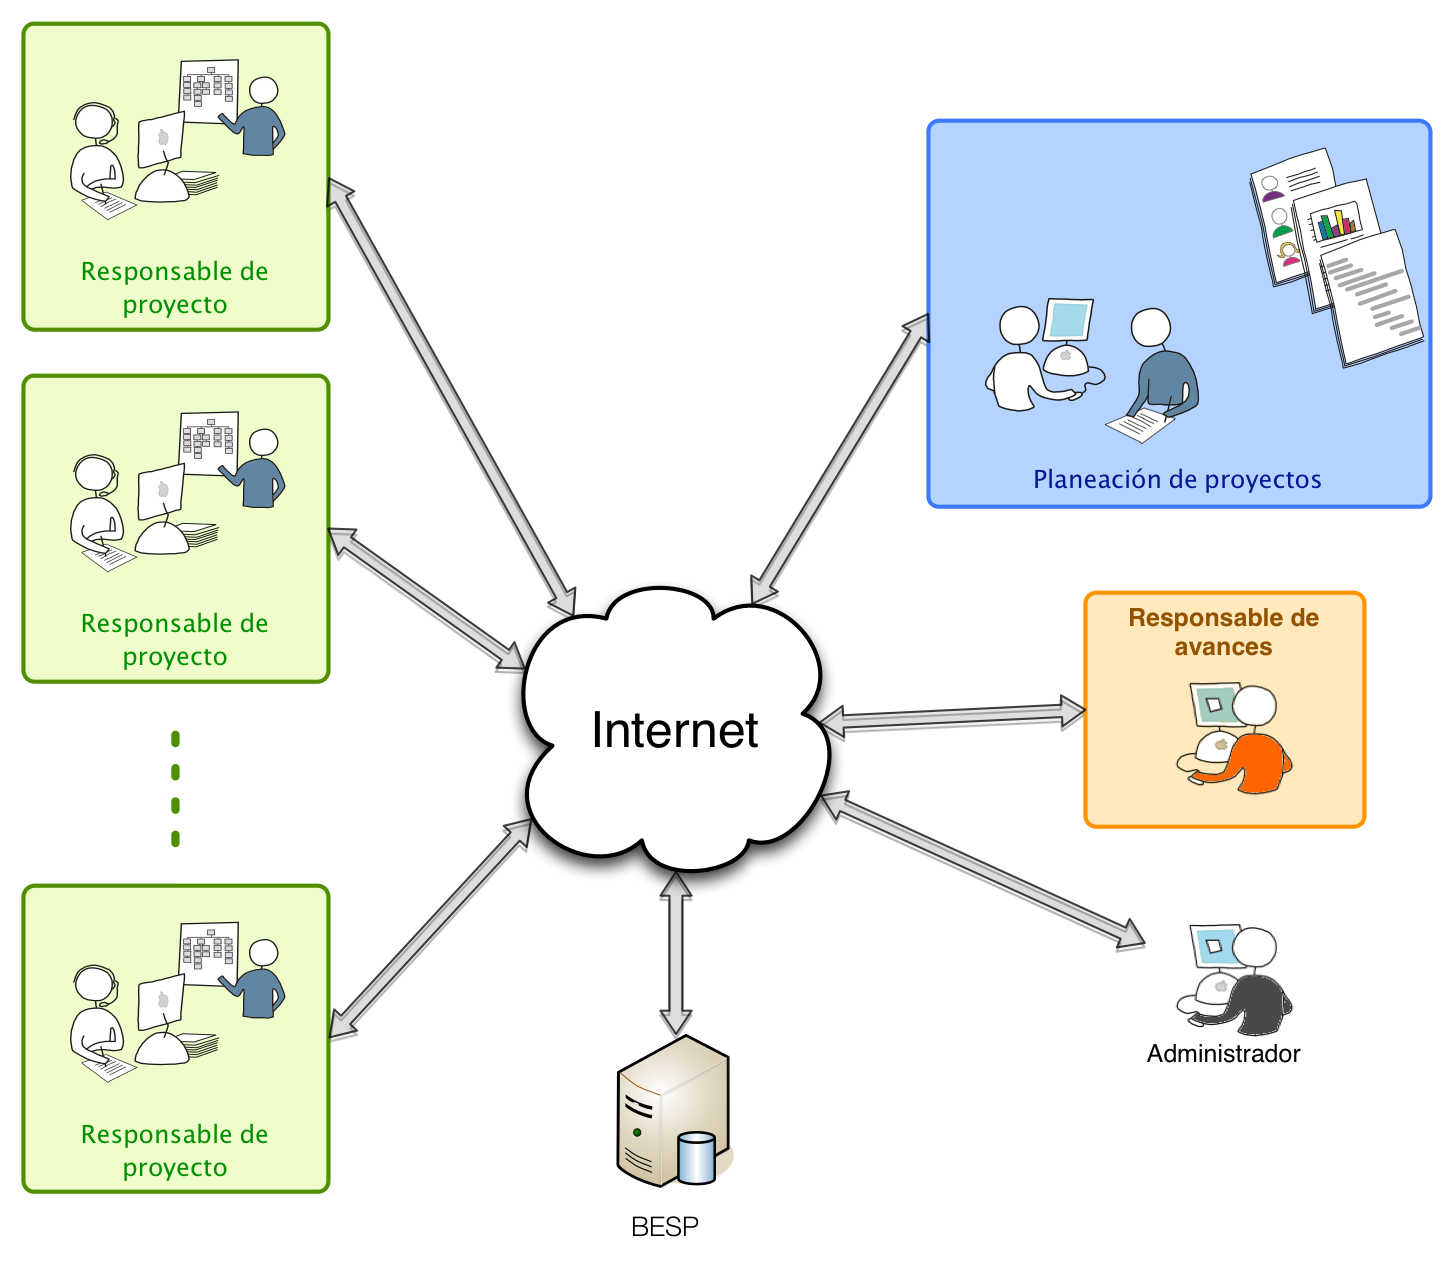
\includegraphics[width=.6\textwidth]{images/arquitectura}}
		\caption{Arquitectura del sistema.}
		\label{fig:arquitectura}
	\end{center}
\end{figure}

En la figura~\ref{fig:arquitectura} se describe la arquitectura general del sistema en la que se destaca el uso de un enfoque basado en micro-servicios, identificando los principales servicios que conforman la propuesta de solución y sus componentes principales.
